\documentclass[bigtut]{tutorial}\usepackage[]{graphicx}\usepackage[]{color}
%% maxwidth is the original width if it is less than linewidth
%% otherwise use linewidth (to make sure the graphics do not exceed the margin)
\makeatletter
\def\maxwidth{ %
  \ifdim\Gin@nat@width>\linewidth
    \linewidth
  \else
    \Gin@nat@width
  \fi
}
\makeatother

\definecolor{fgcolor}{rgb}{0.345, 0.345, 0.345}
\newcommand{\hlnum}[1]{\textcolor[rgb]{0.686,0.059,0.569}{#1}}%
\newcommand{\hlstr}[1]{\textcolor[rgb]{0.192,0.494,0.8}{#1}}%
\newcommand{\hlcom}[1]{\textcolor[rgb]{0.678,0.584,0.686}{\textit{#1}}}%
\newcommand{\hlopt}[1]{\textcolor[rgb]{0,0,0}{#1}}%
\newcommand{\hlstd}[1]{\textcolor[rgb]{0.345,0.345,0.345}{#1}}%
\newcommand{\hlkwa}[1]{\textcolor[rgb]{0.161,0.373,0.58}{\textbf{#1}}}%
\newcommand{\hlkwb}[1]{\textcolor[rgb]{0.69,0.353,0.396}{#1}}%
\newcommand{\hlkwc}[1]{\textcolor[rgb]{0.333,0.667,0.333}{#1}}%
\newcommand{\hlkwd}[1]{\textcolor[rgb]{0.737,0.353,0.396}{\textbf{#1}}}%

\usepackage{framed}
\makeatletter
\newenvironment{kframe}{%
 \def\at@end@of@kframe{}%
 \ifinner\ifhmode%
  \def\at@end@of@kframe{\end{minipage}}%
  \begin{minipage}{\columnwidth}%
 \fi\fi%
 \def\FrameCommand##1{\hskip\@totalleftmargin \hskip-\fboxsep
 \colorbox{shadecolor}{##1}\hskip-\fboxsep
     % There is no \\@totalrightmargin, so:
     \hskip-\linewidth \hskip-\@totalleftmargin \hskip\columnwidth}%
 \MakeFramed {\advance\hsize-\width
   \@totalleftmargin\z@ \linewidth\hsize
   \@setminipage}}%
 {\par\unskip\endMakeFramed%
 \at@end@of@kframe}
\makeatother

\definecolor{shadecolor}{rgb}{.97, .97, .97}
\definecolor{messagecolor}{rgb}{0, 0, 0}
\definecolor{warningcolor}{rgb}{1, 0, 1}
\definecolor{errorcolor}{rgb}{1, 0, 0}
\newenvironment{knitrout}{}{} % an empty environment to be redefined in TeX

\usepackage{alltt}
\unitcode{MATH1005}
        \unitname{Statistics}
        \semester{Summer/Winter/Semester2}
        \sheetnumber7

\usepackage{graphicx}
%\withsolutions
\IfFileExists{upquote.sty}{\usepackage{upquote}}{}
\begin{document}
\lettersfirst

\begin{tutorial}

\begin{displaybox}
Draw a sketch of the appropriate Normal before looking up the Normal table or using R.
\end{displaybox}

\begin{center}
\begin{tabular}{| ll |} \hline
& \\
For a continuous random variable & \\
probability density function (pdf) &   $f(x)$ $ \forall x$  \hspace{.5cm} (often represented as graph) \\
& $f(x) = \frac{dF}{dx} $ \\
cumulative distribution function (CDF) & $F(x) = P(X \leq x) = \int_{-\infty}^{x} f(y) dy$ \\
& $P(X \leq x) = P(X < x)$ \hspace{0.5cm} as $P(X=x) = 0  \hspace{0.2cm} \forall x$ \\
expected value or mean & $E(X) = \int_{x}^{} x f(x) dx$      \\ 
expected value of function  & $E(g(X)) = \int_{x}^{} g(x) f(x) dx$    \\
  & Eg: $E(X^2) = \int_{x}^{} x^2 f(x) dx$    \\
variance & $ Var(X) = E(X^2) - (E(X))^2 $ \\ 
& \\  \hline
\end{tabular}
\end{center}

\begin{displaybox}
{\bf General Normal Distribution}  \\ 
A General Normal random variable $X \sim N(\mu, \sigma^2)$ has mean $\mu$ and variance $\sigma^2$. \\

The pdf is 
$f(x)  =  \frac{1}{  \sqrt{2 \pi \sigma^2}  }  e^{   -\frac{ (x-\mu)^2 }{2 \sigma^2  }    }$ \\ \\

{\bf Standardising a Normal}  \\ 
If $X \sim N(\mu, \sigma^2)$ and $Z \sim N(0, 1)$, then \\
$P( X \leq x) = P \Big( \frac{X-\mu}{\sigma} \leq \frac{x-\mu}{\sigma}  \Big)= P \Big( Z \leq \frac{x-\mu}{\sigma}  \Big)$

\end{displaybox}


\vspace{.5cm}
\begin{questions}

\question
Data collected by Adelaide sports doctor Geoffrey Verrall and AFL sports scientist Jamie Hepner suggest genetics play a bigger part in achieving a top-level football career than skill or desire ... They found those shorter than 180cm could just about forget trying for a place in the elite league - unless they happened to be an indigenous or Pacific Islander player, who thrive on leg speed and lightning reflexes ...
Generally, white Australian males must be tall (about 188cm) to
 make it in the AFL.
{\tiny http://www.heraldsun.com.au/sport/afl/size-matters-at-afl-level/story-e6frf9jf-1226650225771}

\vspace{.5cm}
\begin{parts}
\item What is the average height of Australian males? \\
{\tiny http://www.abs.gov.au/ausstats/abs@.nsf/lookup/4338.0main+features212011-13}

\vspace{.5cm}
\item  Assuming that the population standard deviation is 7 and that heights are Normally distributed, draw a model for the heights of Australian men.


\begin{knitrout}
\definecolor{shadecolor}{rgb}{0.969, 0.969, 0.969}\color{fgcolor}\begin{kframe}
\begin{alltt}
\hlkwd{curve}\hlstd{(}\hlkwd{dnorm}\hlstd{(x,}\hlnum{175.6}\hlstd{,}\hlnum{7}\hlstd{),}\hlkwc{xlim} \hlstd{=} \hlkwd{c}\hlstd{(}\hlnum{140}\hlstd{,} \hlnum{200}\hlstd{),} \hlkwc{xlab}\hlstd{=}\hlstr{"Height"}\hlstd{,} \hlkwc{ylab}\hlstd{=}\hlstr{"Density"}\hlstd{,}
      \hlkwc{main}\hlstd{=}\hlstr{"Australian Men Heights"}\hlstd{,}\hlkwc{col}\hlstd{=}\hlstr{"blue"}\hlstd{)}
\end{alltt}
\end{kframe}
\end{knitrout}

\vspace{.5cm}
\item  AFL's shortest player is Caleb Daniel. How tall is Caleb?  How likely is it to find an Australian man of Caleb's height or shorter?
{\tiny http://www.aflplayers.com.au/article/big-dreams-for-afls-smallest-player/}

\vspace{.5cm}
\item  Adam Goodes is 191cm. How likely is it to find an Australian man of Adam's height or taller?
{\tiny http://www.sydneyswans.com.au/player-profile/adam-goodes}

\vspace{.5cm}
\item If the average height of Australian women is 161.8cm, what proportion of Australian men are below this average?

\end{parts}


\begin{solution}
(a) 175.6cm. \\

(b) $X \sim N(\mu = 75.6, \sigma^2 = 7^2)$. \\

(c) Caleb is 167cm. \\

\begin{knitrout}
\definecolor{shadecolor}{rgb}{0.969, 0.969, 0.969}\color{fgcolor}
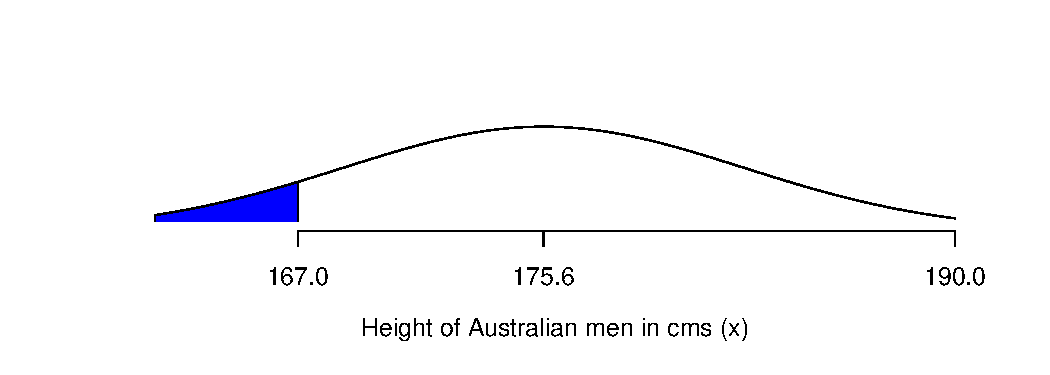
\includegraphics[width=\maxwidth]{figure/unnamed-chunk-3-1} 

\end{knitrout}

$P(X \leq 167) = P(\frac{X-175.6}{7} \leq \frac{167-175.6}{7} ) = P(Z \leq -1.228571) \approx 0.11$

\begin{knitrout}
\definecolor{shadecolor}{rgb}{0.969, 0.969, 0.969}\color{fgcolor}\begin{kframe}
\begin{alltt}
\hlkwd{pnorm}\hlstd{(}\hlnum{167}\hlstd{,}\hlnum{175.6}\hlstd{,}\hlnum{7}\hlstd{)}
\end{alltt}
\begin{verbatim}
## [1] 0.1096163
\end{verbatim}
\begin{alltt}
\hlkwd{pnorm}\hlstd{(}\hlopt{-}\hlnum{1.228571}\hlstd{)}
\end{alltt}
\begin{verbatim}
## [1] 0.1096163
\end{verbatim}
\end{kframe}
\end{knitrout}

(d)

\begin{knitrout}
\definecolor{shadecolor}{rgb}{0.969, 0.969, 0.969}\color{fgcolor}
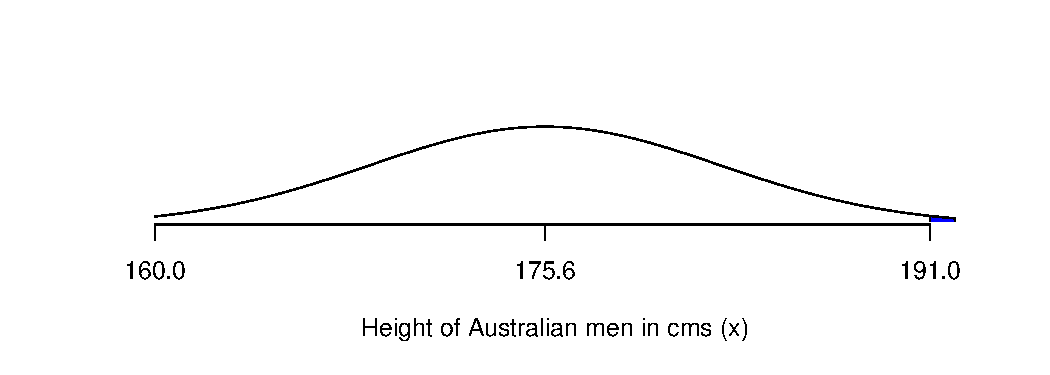
\includegraphics[width=\maxwidth]{figure/unnamed-chunk-5-1} 

\end{knitrout}


$P(X \geq 191) = P(\frac{X-175.6}{7} \geq \frac{191-175.6}{7}) = P(Z \geq 2.2) \approx 0.01$

\begin{knitrout}
\definecolor{shadecolor}{rgb}{0.969, 0.969, 0.969}\color{fgcolor}\begin{kframe}
\begin{alltt}
\hlnum{1}\hlopt{-}\hlkwd{pnorm}\hlstd{(}\hlnum{191}\hlstd{,}\hlnum{175.6}\hlstd{,}\hlnum{7}\hlstd{)}
\end{alltt}
\begin{verbatim}
## [1] 0.01390345
\end{verbatim}
\begin{alltt}
\hlnum{1}\hlopt{-}\hlkwd{pnorm}\hlstd{(}\hlnum{2.2}\hlstd{)}
\end{alltt}
\begin{verbatim}
## [1] 0.01390345
\end{verbatim}
\end{kframe}
\end{knitrout}

(e)

\begin{knitrout}
\definecolor{shadecolor}{rgb}{0.969, 0.969, 0.969}\color{fgcolor}
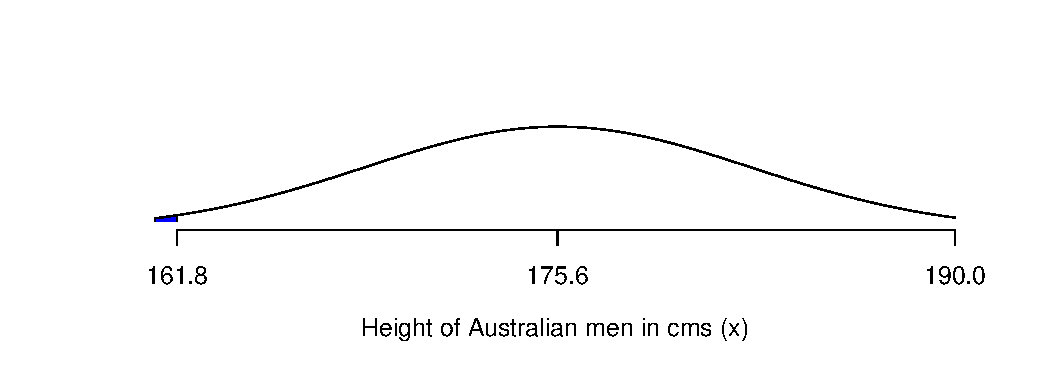
\includegraphics[width=\maxwidth]{figure/unnamed-chunk-7-1} 

\end{knitrout}

$P(X \leq 161.8) = P(\frac{X-175.6}{7} \leq \frac{161.8-175.6}{7}) = P(Z \leq -1.971429) \approx 0.02$

\begin{knitrout}
\definecolor{shadecolor}{rgb}{0.969, 0.969, 0.969}\color{fgcolor}\begin{kframe}
\begin{alltt}
\hlkwd{pnorm}\hlstd{(}\hlnum{161.8}\hlstd{,}\hlnum{175.6}\hlstd{,}\hlnum{7}\hlstd{)}
\end{alltt}
\begin{verbatim}
## [1] 0.02433744
\end{verbatim}
\begin{alltt}
\hlkwd{pnorm}\hlstd{(}\hlopt{-}\hlnum{1.971429}\hlstd{)}
\end{alltt}
\begin{verbatim}
## [1] 0.02433741
\end{verbatim}
\end{kframe}
\end{knitrout}


\end{solution}







\question Standardising Normal Distribution \\

In 2011-12, the Australian Bureau of Statistics reported a tendency for high levels of sedentary behaviour across the Australian adult population, with Australian adults spending an average of 13 hours a week watching TV. \\
{\tiny http://www.abs.gov.au/ausstats/abs@.nsf/lookup/4364.0.55.004Media\%20Release22011-12} \\

Let $X$ be the number of hours per week spent watching TV by an Australian adult. Model $X$ by a Normal with standard deviation $\sigma = 2$ hours.  \\

\begin{parts}
\part Plot the curve. 

\begin{knitrout}
\definecolor{shadecolor}{rgb}{0.969, 0.969, 0.969}\color{fgcolor}\begin{kframe}
\begin{alltt}
\hlkwd{curve}\hlstd{(}\hlkwd{dnorm}\hlstd{(x,}\hlnum{13}\hlstd{,}\hlnum{2}\hlstd{),}\hlnum{10}\hlstd{,}\hlnum{20}\hlstd{,} \hlkwc{main}\hlstd{=}\hlstr{"Weekly hours of TV watching by Australian adults"}\hlstd{)}
\end{alltt}
\end{kframe}
\end{knitrout}

\vspace{.5cm}
\part For an Australian adult chosen at random, find the probability that the person watches between 12 and 16 hours of TV per week.

\vspace{.5cm}
\part What is the 90\% percentile for weekly TV watching by Australian adults?

\begin{knitrout}
\definecolor{shadecolor}{rgb}{0.969, 0.969, 0.969}\color{fgcolor}\begin{kframe}
\begin{alltt}
\hlkwd{qnorm}\hlstd{(}\hlnum{0.9}\hlstd{,}\hlnum{13}\hlstd{,}\hlnum{2}\hlstd{)}
\end{alltt}
\begin{verbatim}
## [1] 15.5631
\end{verbatim}
\end{kframe}
\end{knitrout}
\end{parts}


\begin{solution}
$X \sim N(\mu = 13, \sigma^2 = 4)$.  \\

(b)
\begin{knitrout}
\definecolor{shadecolor}{rgb}{0.969, 0.969, 0.969}\color{fgcolor}
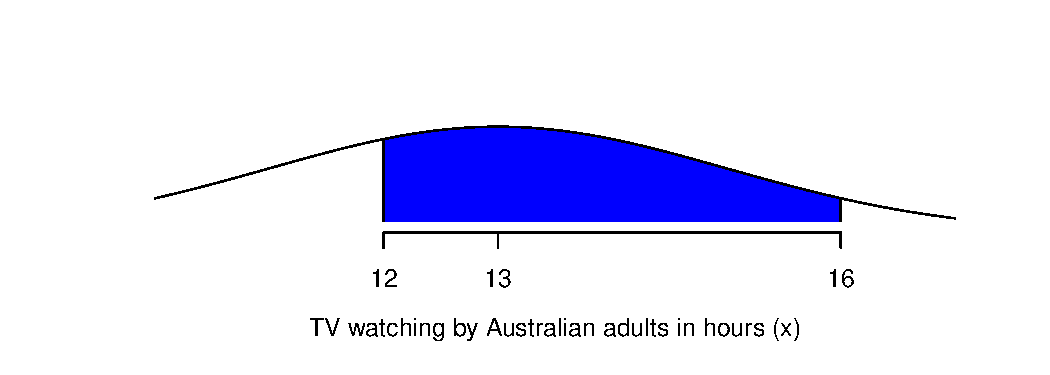
\includegraphics[width=\maxwidth]{figure/unnamed-chunk-11-1} 

\end{knitrout}

$P(12 < X < 16) = P \big(\frac{12-13}{2} < \frac{X-13}{2}  < \frac{16-13}{2} \big) = P(-0.5 < Z < 1.5) = \Phi(1.5) - \Phi(-0.5) = 0.6246553 \approx 0.6$. \\

\begin{knitrout}
\definecolor{shadecolor}{rgb}{0.969, 0.969, 0.969}\color{fgcolor}\begin{kframe}
\begin{alltt}
\hlkwd{pnorm}\hlstd{(}\hlnum{16}\hlstd{,}\hlnum{13}\hlstd{,}\hlnum{2}\hlstd{)} \hlopt{-} \hlkwd{pnorm}\hlstd{(}\hlnum{12}\hlstd{,}\hlnum{13}\hlstd{,}\hlnum{2}\hlstd{)}
\end{alltt}
\begin{verbatim}
## [1] 0.6246553
\end{verbatim}
\begin{alltt}
\hlkwd{pnorm}\hlstd{(}\hlnum{1.5}\hlstd{)}\hlopt{-}\hlkwd{pnorm}\hlstd{(}\hlopt{-}\hlnum{0.5}\hlstd{)}
\end{alltt}
\begin{verbatim}
## [1] 0.6246553
\end{verbatim}
\end{kframe}
\end{knitrout}

\vspace{.5cm}
(c) We want $q$ such that $P(X < q) = 0.9$. \\
So $0.9 = P(X < q) = P \big(\frac{X-13}{2}  < \frac{q-13}{2} \big) = P(Z < \frac{q-13}{2})$. \\
As $0.9 = P(Z < 1.28)$ (from table or R), we solve $1.28 = \frac{q-13}{2}$, which gives $q = 2*1.28 + 13 = 15.56$.

\begin{knitrout}
\definecolor{shadecolor}{rgb}{0.969, 0.969, 0.969}\color{fgcolor}\begin{kframe}
\begin{alltt}
\hlkwd{qnorm}\hlstd{(}\hlnum{0.9}\hlstd{,}\hlnum{13}\hlstd{,}\hlnum{2}\hlstd{)}
\end{alltt}
\begin{verbatim}
## [1] 15.5631
\end{verbatim}
\end{kframe}
\end{knitrout}

\vspace{.5cm}
Alternatively, we can use R directly:
\begin{knitrout}
\definecolor{shadecolor}{rgb}{0.969, 0.969, 0.969}\color{fgcolor}\begin{kframe}
\begin{alltt}
\hlkwd{qnorm}\hlstd{(}\hlnum{0.9}\hlstd{)}
\end{alltt}
\begin{verbatim}
## [1] 1.281552
\end{verbatim}
\end{kframe}
\end{knitrout}


\end{solution}




\question Expectation of Normal Distribution \\

Suppose that $X$ is the breaking strength of a rope in pounds, with distribution $N(100,16)$. Each 30 metre coil of rope brings a return of $\$25$ provided $X > 95$. If $X\leq 95$ then the rope is used for a different purpose and a return of only $ \$10 $ per coil is made. Find the expected return per coil. 



\begin{solution}
$X = \text{the breaking strength of a rope in pounds} \sim N(100,16)$.  \\

(1) Good quality rope : If $P(X> 95)$ then \$25 return. \\

$P(X > 95) = P \big( \frac{X-100}{4} > \frac{95-100}{4} \big) = P(Z > -5/4) = P(Z < 5/4) = \Phi(5/4) = 0.8943$. \\

(2) Poor quality rope : If $P(X< 95)$ then \$10 return. \\

$P(X < 95) = 1- P(X > 95) = 0.1057$. \\

Hence expected return per coil of rope is: \\
$E(X) = P(X>95) \times \$25 + P(X<95) \times \$10 = 
0.8943 \times \$25 + 0.1057 \times \$10 = \$23.4145 $.
\end{solution}





\newpage
\hspace{-1cm}  {\bf Extra Questions}


\question Standard Normal Probabilities  \\

Given $Z \sim N (0,1)$. \\

\begin{parts}

\part Plot $Z$.

\begin{knitrout}
\definecolor{shadecolor}{rgb}{0.969, 0.969, 0.969}\color{fgcolor}\begin{kframe}
\begin{alltt}
\hlkwd{curve}\hlstd{(}\hlkwd{dnorm}\hlstd{(x),}\hlopt{-}\hlnum{3}\hlstd{,}\hlnum{3}\hlstd{)}   \hlcom{#Plots Standard Normal from -3 to 3.}
\end{alltt}
\end{kframe}
\end{knitrout}

\part From looking at the plot, estimate $P(Z \leq 1)$ and $P(Z \leq -1)$. Check by looking up the Normal table, and using R.

\begin{knitrout}
\definecolor{shadecolor}{rgb}{0.969, 0.969, 0.969}\color{fgcolor}\begin{kframe}
\begin{alltt}
\hlkwd{pnorm}\hlstd{(}\hlnum{1}\hlstd{)}   \hlcom{#Calculates P(Z < 1)}
\end{alltt}
\begin{verbatim}
## [1] 0.8413447
\end{verbatim}
\end{kframe}
\end{knitrout}

\part Fill out the following table. What do these probabilities represent?

\begin{center}
\begin{tabular}{| c | c | c |} \hline
$P( -1 \leq Z \leq 1)$ & $P( -2 \leq Z \leq 2)$ & $P( -3 \leq Z \leq 3)$ \\ \hline
0.68 & & \\ \hline
\end{tabular}
\end{center}

\begin{knitrout}
\definecolor{shadecolor}{rgb}{0.969, 0.969, 0.969}\color{fgcolor}\begin{kframe}
\begin{alltt}
\hlkwd{pnorm}\hlstd{(}\hlnum{1}\hlstd{)}\hlopt{-}\hlkwd{pnorm}\hlstd{(}\hlopt{-}\hlnum{1}\hlstd{)}
\end{alltt}
\end{kframe}
\end{knitrout}

\part 
Using the Normal table, find the values of $a$, $b$ and $c$ such that
$P(Z \leq a)=0.7291, P(Z > b)=0.10$ and $P(|Z| <c)=0.90$. Check your answers in R.

\begin{knitrout}
\definecolor{shadecolor}{rgb}{0.969, 0.969, 0.969}\color{fgcolor}\begin{kframe}
\begin{alltt}
\hlkwd{qnorm}\hlstd{(}\hlnum{0.7291}\hlstd{)}   \hlcom{#Calculates a st P(Z < a) = 0.7291}
\end{alltt}
\end{kframe}
\end{knitrout}
\end{parts}


\begin{solution}
(a) From Normal tables,
$P(Z \leq 1) = 0.8413$ \\
$P(Z \leq -1) = 1- P(Z \leq 1) = 0.1587$. \\

(b)
\begin{tabular}{| c | c | c |} \hline
$P( -1 \leq Z \leq 1)$ & $P( -2 \leq Z \leq 2)$ & $P( -3 \leq Z \leq 3)$ \\ \hline
0.6827 or 0.68 & 0.9545 or 0.95 & 0.9973  or 0.99 \\ \hline
\end{tabular}

 \vspace{.5cm}
Comment: This table represents the probability of being 1,2 and 3 standard deviations away from the mean. 
Eg The probability of being within 1 standard deviation of the mean is approximately $68 \%$. \\

(c) 
Using the Normal table, \\
if $P(Z \leq a) = 0.7291$, then  $a = 0.6101$ \\
if $P(Z > b) = 0.10$, then $P(Z < b) = 0.90$, so $b = 1.2816$ \\
if $P(|Z| <c) = 0.90$, then $P(Z <c)=0.95$, hence
$c =  1.645$ \\
\end{solution}


\question Normal Distribution \\

Each day random samples of a city's water supply are analysed and the concentration of fluoride (parts per million, ppm) is measured. It is found that the distribution of this concentration is approximately normal with mean of 1.3 ppm and a standard deviation of 0.15 ppm. \\

\begin{parts}
\part 
On what proportion of days is the concentration  between 1.45 and 1.53 ppm?
\part 
What is the 80th percentile of the distribution? What does this represent?

\end{parts}



\begin{solution}
$X = \text{the concentration of fluoride} \sim N(1.3, 0.15^2)$. \\

(a)
$P(1.45 \leq X \leq 1.53) = P \big( \frac{1.45-1.3}{0.15} \leq \frac{X-1.3}{0.15} \leq \frac{1.53-1.3}{0.15} \big) = P(1 < Z < 1.53) = \Phi(1.53)-\Phi(1) = 0.9370 - 0.8413 = 0.0957$ \\

\begin{knitrout}
\definecolor{shadecolor}{rgb}{0.969, 0.969, 0.969}\color{fgcolor}\begin{kframe}
\begin{alltt}
\hlkwd{pnorm}\hlstd{(}\hlnum{1.53}\hlstd{,}\hlnum{1.3}\hlstd{,}\hlnum{0.15}\hlstd{)}\hlopt{-}\hlkwd{pnorm}\hlstd{(}\hlnum{1.45}\hlstd{,}\hlnum{1.3}\hlstd{,}\hlnum{0.15}\hlstd{)}
\end{alltt}
\begin{verbatim}
## [1] 0.09605838
\end{verbatim}
\end{kframe}
\end{knitrout}

\vspace{.5cm}
(b)
We want to find $q$ such that $P(X < q) = 0.8$.\\

$P(X < q) = P \big( \frac{X-1.3}{0.15} < \frac{q-1.3}{0.15} \big) = P(Z <\frac{q-1.3}{0.15}) = 0.8$. \\

From looking up Normal tables, we find that $\frac{q-1.3}{0.15} = 0.8416$. So $q = 1.4262$. \\

Represents: We expect the level of fluoride to be less than 1.4262 80\% of the time. \\

\begin{knitrout}
\definecolor{shadecolor}{rgb}{0.969, 0.969, 0.969}\color{fgcolor}\begin{kframe}
\begin{alltt}
\hlkwd{pnorm}\hlstd{(}\hlnum{1.4262}\hlstd{,}\hlnum{1.3}\hlstd{,}\hlnum{0.15}\hlstd{)}  \hlcom{# which is approximately 80%}
\end{alltt}
\begin{verbatim}
## [1] 0.7999194
\end{verbatim}
\end{kframe}
\end{knitrout}
\end{solution}



\question Continuous Distribution by hand \\

A random variable $X$ has the following CDF:
\[ F(x) =      \left\{     \begin{array}{ll} 0        & x \leq 0  \\
                                                         x/2     & x \in (0,2)  \\
                                                         1        & x \geq 2 
  		      \end{array}    \right.  \]


\begin{parts}
\part Sketch the CDF.
\part Find the pdf and sketch it.
\part Calculate $E(X)$ and $Var(X)$. Does this match up with your sketches?
\end{parts}


\begin{solution}
(a) Check your hand drawn sketch against this R output:

\begin{knitrout}
\definecolor{shadecolor}{rgb}{0.969, 0.969, 0.969}\color{fgcolor}
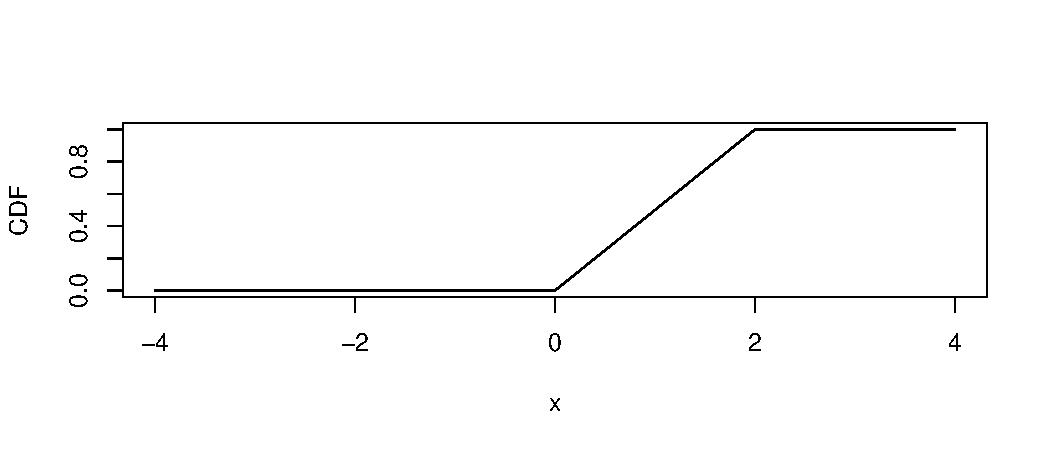
\includegraphics[width=\maxwidth]{figure/unnamed-chunk-21-1} 

\end{knitrout}


(b) 
To get the pdf, we differentiate the CDF. Hence,
\[ f(x) =      \left\{     \begin{array}{ll} 0        & x \leq 0  \\
                                                         \frac{1}{2}     & x \in (0,2)  \\
                                                         0        & x \geq 2 
  		      \end{array}    \right.  \]
giving
\[ f(x) =      \left\{     \begin{array}{ll}                                                      \frac{1}{2}     & x \in (0,2)  \\
                                                         0        & \text{otherwise} 
    	      \end{array}    \right.  \]

Again, check your hand drawn sketch against this R output:

\begin{knitrout}
\definecolor{shadecolor}{rgb}{0.969, 0.969, 0.969}\color{fgcolor}
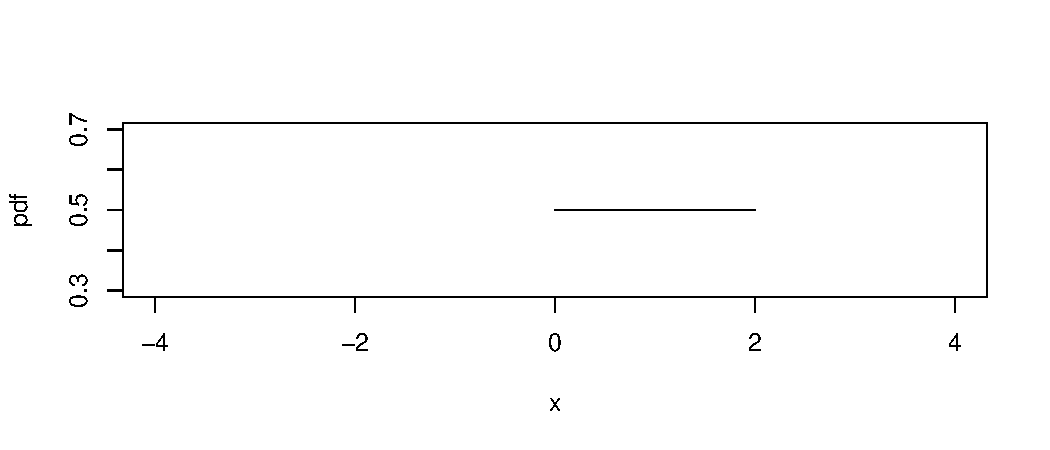
\includegraphics[width=\maxwidth]{figure/unnamed-chunk-22-1} 

\end{knitrout}


(c)
$E(X) = \int_{-\infty}^{\infty} x f(x) dx = \frac{1}{2} \int_{0}^{2}x dx = \frac{1}{2} \big[ \frac{x^2}{2} \big]_{0}^{2}  = 1$\\

Comment: As the pdf is symmetric, we expect the mean at $x=1$. \\

$E(X^2) = \int_{-\infty}^{\infty} x^2 f(x) dx = \frac{1}{2} \int_{0}^{2}x^2 dx = \frac{1}{2} \big[ \frac{x^3}{3} \big]_{0}^{2}  = 8/6$\\

Hence $Var(X) = 8/6 - (1)^2 = 1/3$, and $SD(X) \approx 0.58$.  \\

Comment: Looking at the pdf, it seems reasonable that the standard deviation would be 0.58.
(The mean is 1 and the full range of data is only 2).

\end{solution}


\question Normal Probabilities  \\

Given $X \sim N (5,4)$. \\

\begin{parts}

\part
What is  $P(X=1)$?  

\part Calculate $P(X \leq 1)$   and  $P(-2 \leq X \leq 1)$.

\part Use R to confirm your answers.

\begin{knitrout}
\definecolor{shadecolor}{rgb}{0.969, 0.969, 0.969}\color{fgcolor}\begin{kframe}
\begin{alltt}
\hlkwd{pnorm}\hlstd{(}\hlnum{1}\hlstd{,}\hlnum{5}\hlstd{,}\hlnum{2}\hlstd{)}      \hlcom{#Calculates P(X <=1)}
\end{alltt}
\begin{verbatim}
## [1] 0.02275013
\end{verbatim}
\end{kframe}
\end{knitrout}
\end{parts}

\begin{solution}
(a)
For any continuous distribution, $P(X=x) = 0$  for all $x$. \\

(b) 
$P(X \leq 1) = P \big( \frac{X-5}{2} \leq \frac{1-5}{2} \big) = P(Z \leq -2) = 1- P(Z \leq 2) = 1- \Phi(2) = 0.0228$  \\ 
$P(-2 \leq X \leq 1) = P(\frac{-2-5}{2} \leq \frac{X-5}{2} \leq \frac{1-5}{2}) = P(-3.5 \leq Z \leq -2) =
P(2 \leq Z \leq 3.5) = \Phi(3.5)-\Phi(2) = 0.0226$.

(c)
\begin{knitrout}
\definecolor{shadecolor}{rgb}{0.969, 0.969, 0.969}\color{fgcolor}\begin{kframe}
\begin{alltt}
\hlkwd{pnorm}\hlstd{(}\hlnum{1}\hlstd{,}\hlnum{5}\hlstd{,}\hlnum{2}\hlstd{)}
\end{alltt}
\begin{verbatim}
## [1] 0.02275013
\end{verbatim}
\begin{alltt}
\hlkwd{pnorm}\hlstd{(}\hlopt{-}\hlnum{2}\hlstd{)}
\end{alltt}
\begin{verbatim}
## [1] 0.02275013
\end{verbatim}
\begin{alltt}
\hlkwd{pnorm}\hlstd{(}\hlnum{3.5}\hlstd{)}\hlopt{-}\hlkwd{pnorm}\hlstd{(}\hlnum{2}\hlstd{)}
\end{alltt}
\begin{verbatim}
## [1] 0.0225175
\end{verbatim}
\end{kframe}
\end{knitrout}
\end{solution}


\end{questions}
\end{tutorial}
\end{document}

